\documentclass[11pt,conference]{IEEEtran}
\IEEEoverridecommandlockouts

\usepackage[utf8]{inputenc}
\usepackage[T1]{fontenc}
\usepackage{amsmath,amssymb,amsfonts}
\usepackage{graphicx}
\usepackage{cite}
\usepackage{booktabs}
\usepackage{array}
\usepackage{url}
\usepackage{balance}
\usepackage{tikz}
\usetikzlibrary{shapes.geometric,arrows.meta,positioning,fit,backgrounds}
\usepackage{algorithm}
\usepackage{algpseudocode}
\usepackage[letterpaper,top=0.75in,bottom=1.00in,left=0.75in,right=0.75in]{geometry}

% Spacing parameters calibrated for 6-page IEEE conference target
\setlength{\columnsep}{0.22in}
\setlength{\textfloatsep}{5pt plus 2pt minus 1pt}
\setlength{\floatsep}{4pt plus 1pt minus 1pt}
\setlength{\dbltextfloatsep}{6pt plus 2pt minus 1pt}
\setlength{\dblfloatsep}{4pt plus 1pt minus 1pt}
\setlength{\abovecaptionskip}{2.5pt plus 1pt minus 1pt}
\setlength{\belowcaptionskip}{2.5pt plus 1pt minus 1pt}
\setlength{\abovedisplayskip}{2.5pt plus 1pt minus 1pt}
\setlength{\belowdisplayskip}{2.5pt plus 1pt minus 1pt}
\setlength{\abovedisplayshortskip}{1pt plus 1pt minus 1pt}
\setlength{\belowdisplayshortskip}{1pt plus 1pt minus 1pt}

% Configure graphics search path for publication assets
\graphicspath{{figures/}}

% TikZ styles for architecture diagram (optimized for single-column width)
\tikzset{
  netbox/.style={draw=blue!70,fill=blue!5,rounded corners=2pt,
      text width=4.8cm,align=center,font=\small,inner sep=2.5pt,minimum height=0.55cm},
  modeA/.style={draw=teal!70,fill=teal!6,rounded corners=2pt,
      text width=3.1cm,align=center,font=\small,inner sep=2.5pt,minimum height=0.60cm},
  modeB/.style={draw=orange!70,fill=orange!8,rounded corners=2pt,
      text width=3.1cm,align=center,font=\small,inner sep=2.5pt,minimum height=0.60cm},
  extbox/.style={draw=gray!70,fill=gray!6,rounded corners=2pt,
      text width=3.1cm,align=center,font=\small,inner sep=2.5pt,minimum height=0.50cm},
  altbox/.style={draw=violet!70,fill=violet!6,rounded corners=2pt,
      text width=3.1cm,align=center,font=\small,inner sep=2.5pt,minimum height=0.60cm},
  arr/.style={-{Latex[length=3.5pt,width=2.5pt]},line width=0.5pt,gray!70},
}

\title{Design and Empirical Evaluation of a Two-Wheeler-Aware Routing Framework for Urban Road Networks}

\author{
\IEEEauthorblockA{
\textbf{Anirudh R}, \textbf{Vikhyath K B}, \textbf{A Nikhil Kumar}, \textbf{Shwetha M D}, \textbf{Akshath G}, \textbf{Chiranandan T M}\\
Department of Computer Science and Engineering, BNM Institute of Technology, Bengaluru, India\\
Emails: \texttt{anirudhraju7@gmail.com}, \texttt{vikhyathkb@bnmit.in}, \texttt{\{23cse100, 23cse167, 23cse186\}@bnmit.in}, \texttt{shwetha.0116@gmail.com}}
}

\begin{document}

\maketitle

% ============================================================
% ABSTRACT
% ============================================================

\begin{abstract}
Commercial navigation engines designed for passenger cars inadequately serve motorized two-wheelers in dense South Asian cities, where riders encounter frequent sharp turns and saturated arterials.
This paper presents a two-wheeler-aware routing framework that combines turn-aware state-expanded $A^*$ search with two operational modes (Shortest and Dynamic) and a perpendicular-offset alternative-route generator.
The search model incorporates discrete turn penalties, road-class impedance, and an admissible Haversine heuristic.
Across 25 representative Bengaluru corridors (Experiment E), the offset generator yields valid alternatives satisfying detour $\le 1.20$ and edge-overlap $\le 0.70$ on 22 corridors (88.0\%), achieving a mean pairwise diversity of 0.5605 on successful corridors (measured).
A descriptive five-corridor benchmark against Yen's algorithm indicates a coverage-versus-diversity trade-off: filtered Yen provides higher route coverage (2.4 vs.\ 1.2 routes), whereas offset alternatives exhibit greater topological separation where both succeed (mean Jaccard diversity 0.58 vs.\ 0.35, $n=3$).
A four-pair manual pilot documents comparative metrics across the framework, Google Maps, and Waze without asserting platform ranking.
Repeated GPS journeys ($n=5$ rides across three days) confirm that Day~1 and Day~3 trajectories follow near-identical paths (mean deviation 3.4~m morning, 2.9~m afternoon; measured).
All findings are descriptive measurements; no travel-time savings, safety benefits, or platform superiority are claimed.
\end{abstract}

\begin{IEEEkeywords}
Two-wheeler routing, alternative routes, perpendicular offset, K-shortest paths, urban road networks, OpenStreetMap, GPS trajectory analysis.
\end{IEEEkeywords}

% ============================================================
% I. INTRODUCTION
% ============================================================

\section{Introduction}

Motorized two-wheelers constitute a dominant share of vehicular traffic in Indian metropolitan areas \cite{kotagi2020modeling,das2019modeling}.
In dense road networks such as Bengaluru, riders navigate congested arterials, complex intersections, and hazardous acute turns across opposing traffic.
Standard routing engines, designed primarily for passenger cars, frequently direct two-wheelers onto congested arterials or paths requiring difficult turning maneuvers \cite{kumar2025realtime,luxen2011realtime}.

To address these challenges, this paper presents an end-to-end two-wheeler navigation framework.
The framework couples a turn-aware state-expanded $A^*$ routing algorithm with live-traffic congestion avoidance and a geometric perpendicular-offset alternative-route generator.
Search states track directed edge transitions, penalizing acute angular deflections and prioritizing local secondary links over congested multilane arterials.
In parallel, lateral intermediate waypoints generate topologically distinct alternatives while enforcing strict detour and overlap bounds.

The contributions of this paper are:
\begin{enumerate}
\item A two-mode routing framework (Shortest and Dynamic) integrating turn-aware state-expanded $A^*$ search, live congestion avoidance, and snapshot persistence.
\item A perpendicular-offset alternative-route generator with bounded detour ($\le 1.20$) and edge-overlap ($\le 0.70$) filtering, returning up to $K=3$ alternatives from 12 lateral waypoint candidates.
\item An empirical evaluation across 25 Bengaluru corridors and a descriptive five-corridor comparison against Yen's K-shortest paths (Experiment E).
\item A four-pair manual pilot comparing framework, Google Maps, and Waze predictions from visual map interfaces without API reliance.
\item Real-world GPS trajectory analysis across five repeat rides over three days, evaluating spatial path consistency and stopped-time sensitivity.
\end{enumerate}

% ============================================================
% II. RELATED WORK
% ============================================================

\section{Related Work}

\noindent\textbf{Turn-Aware Shortest Path Routing:}
Standard shortest-path algorithms evaluate traversal costs at graph vertices and cannot represent turn-dependent penalties without network expansion \cite{winter2002modeling,geisberger2011efficient}.
State-expanded formulations map directed edges to search states, supporting discrete angular penalties during edge relaxation \cite{winter2002modeling}.
Contraction Hierarchies and Customizable Contraction Hierarchies extend hierarchical routing to turn costs, but customising heterogeneous cost models in large urban networks introduces significant preprocessing complexity \cite{geisberger2011efficient,bast2016route,delling2017customizable}.

\noindent\textbf{Alternative Route Generation:}
Yen's algorithm \cite{yen1971finding} computes the $K$ loopless shortest paths in ascending cost order.
On dense planar grids, successive Yen paths typically deviate by only minor block detours, resulting in high edge overlap and minimal topological diversity.
Plateau and $T$-restricted alternative graphs \cite{abraham2013alternative} enforce separation but require complex hierarchical preprocessing.
Lateral waypoint placement offers a lightweight alternative by displacing search midpoints perpendicularly from the origin-destination chord \cite{asvial2020entropy}.

\noindent\textbf{Urban Mobility and Commercial Systems:}
Commercial navigation services optimize routes primarily for passenger cars \cite{luxen2011realtime,kumar2025realtime}.
Studies on motorcycle route choice under real-time information \cite{fadilah2024identifying} and multi-criteria ranking \cite{asvial2020entropy} omit physical turning penalties during graph search.
Kinematic investigations verify that two-wheelers exhibit distinctive lane-filtering and lateral movement behaviors in mixed traffic \cite{kotagi2020modeling,das2019modeling,promraksa2022lane}.
OSMnx \cite{boeing2017osmnx} provides network extraction tools, while Kumar et al.\ \cite{kumar2025realtime} document recurrent congestion in Bengaluru, motivating two-wheeler bypass modeling.

% ============================================================
% III. FRAMEWORK DESIGN
% ============================================================

\section{Framework Design}

\subsection{Architecture Overview}

\begin{figure}[t]
\centering
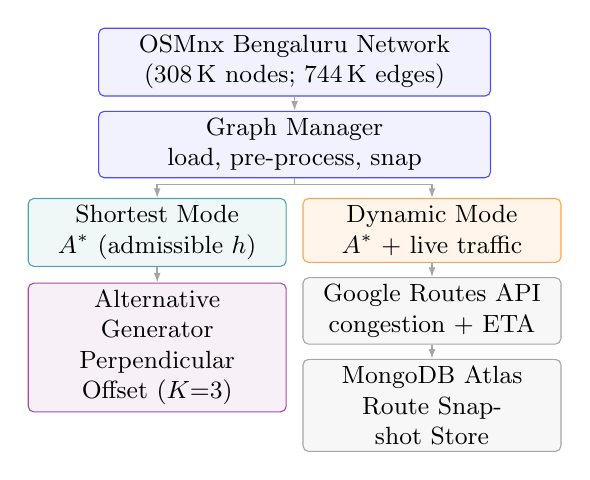
\begin{tikzpicture}[node distance=0.22cm and 0.28cm]
  \node[netbox] (osm) {OSMnx Bengaluru Network\\(308\,K nodes; 744\,K edges)};
  \node[netbox, below=0.18cm of osm] (gm) {Graph Manager\\load, pre-process, snap};

  \node[modeA, below left=0.25cm and 0.10cm of gm.south] (sh)
    {Shortest Mode\\$A^*$ (admissible $h$)};
  \node[modeB, below right=0.25cm and 0.10cm of gm.south] (dyn)
    {Dynamic Mode\\$A^*$ + live traffic};

  \node[altbox, below=0.20cm of sh] (off)
    {Alternative Generator\\Perpendicular Offset ($K{=}3$)};
  \node[extbox, below=0.18cm of dyn] (gapi)
    {Google Routes API\\congestion + ETA};
  \node[extbox, below=0.18cm of gapi] (mdb)
    {MongoDB Atlas\\Route Snapshot Store};

  \draw[arr] (osm) -- (gm);
  \draw[arr] (gm.south) -- ++(0,-0.08) -| (sh.north);
  \draw[arr] (gm.south) -- ++(0,-0.08) -| (dyn.north);
  \draw[arr] (sh)  -- (off);
  \draw[arr] (dyn) -- (gapi);
  \draw[arr] (gapi) -- (mdb);
\end{tikzpicture}
\caption{System architecture. GraphManager constructs the road network. Shortest mode runs turn-aware $A^*$. Dynamic mode incorporates live congestion polylines and retrieves traffic-aware ETAs via sampled waypoints. The alternative generator wraps the core search engine.}
\label{fig:architecture}
\end{figure}

The framework operates on an OpenStreetMap graph of Bengaluru (308,643 vertices; 744,216 raw edges; 740,822 distinct ordered pairs after parallel-edge collapse).
Shortest Mode executes turn-aware state-expanded $A^*$ search using static road-class impedance and angular turn penalties.
Dynamic Mode queries the Google Routes API (TWO\_WHEELER travel mode, TRAFFIC\_AWARE preference) to identify congested segments, applies multiplied traversal penalties to corresponding vertices, and re-solves $A^*$.
Up to 20 sampled via-waypoints along the calculated path are transmitted back to the API to retrieve a traffic-aware ETA, and route metadata are persisted to MongoDB Atlas.

\textit{Independence note:} Because Dynamic mode ETAs are retrieved by submitting the framework's own route geometry to the Google Routes API, the framework and Google are not independent duration estimators. Their ETAs cannot be compared as competing measurements.

\subsection{Routing Cost Model}

In the state-expanded search graph, each state $s = (u, v)$ represents directed traversal of edge $(u, v)$.
This edge-state formulation allows evaluating the deflection angle $\theta$ between incoming edge $(u, v)$ and candidate outgoing edge $(v, w)$ during vertex relaxation.
The traversal cost of transitioning from state $(u,v)$ to $(v,w)$ is:
\begin{equation}
  c\bigl((u,v)\to(v,w)\bigr) = c_\mu(v,w) + P_\text{turn}(u,v,w)
  \label{eq:astar_cost}
\end{equation}
where $c_\mu(v,w) = \ell(v,w)\cdot\mu(v,w)$ is the impedance-weighted edge cost ($\ell$ is physical length in meters; $\mu \ge 0.80$ is the road-class multiplier).
The impedance model prioritizes tertiary and residential links over saturated primary arterials.
The discrete turn penalty $P_\text{turn}$ adds 25.0~m for turns $\ge 60^\circ$, 8.0~m for $30^\circ$--$60^\circ$, and 0.0~m otherwise.
The heuristic function is:
\begin{equation}
  h(v) = 0.80 \cdot d_\text{Haversine}(v,\, t)
  \label{eq:heuristic}
\end{equation}
Because $\mu(e) \ge 0.80$ across all edges and turn penalties are strictly non-negative, $h(v)$ never overestimates remaining cost, ensuring an admissible and consistent $A^*$ search.

In Dynamic mode, vertices along congested segments incur a multiplied traversal cost:
\begin{equation}
  \mu_\text{cong}(e) = 25 \cdot \mu(e), \quad u \in \mathcal{C} \text{ or } v \in \mathcal{C}
  \label{eq:congestion}
\end{equation}
where $\mathcal{C}$ denotes the set of congested network vertices.

\subsection{Perpendicular-Offset Waypoint Generation}

For origin $O=(\varphi_O,\lambda_O)$ and destination $D=(\varphi_D,\lambda_D)$ in decimal degrees, the forward azimuth of the chord is:
\begin{equation}
  \beta = \arctan2\!\left(\sin\Delta\lambda\cos\varphi_D,\;
         \cos\varphi_O\sin\varphi_D - \sin\varphi_O\cos\varphi_D\cos\Delta\lambda\right) \bmod 360^\circ
  \label{eq:bearing}
\end{equation}

At each chord fraction $\alpha \in \{0.33, 0.50, 0.67\}$, an intermediate base point is interpolated linearly:
\begin{equation}
  p_b(\alpha) = \bigl(\varphi_O + \alpha(\varphi_D-\varphi_O),\;\lambda_O + \alpha(\lambda_D-\lambda_O)\bigr)
  \label{eq:chord_point}
\end{equation}

Base points are laterally displaced using spherical destination equations.
For perpendicular directions $\beta_\perp \in \{\beta{+}90^\circ,\;\beta{-}90^\circ\}$ and lateral distances $d \in \{150~\text{m}, 300~\text{m}\}$:
\begin{align}
  \varphi_w &= \arcsin\!\left(\sin\varphi_b\cos\tfrac{d}{R} + \cos\varphi_b\sin\tfrac{d}{R}\cos\beta_\perp\right) \label{eq:dest_lat}\\
  \lambda_w &= \lambda_b + \arctan2\!\left(\sin\beta_\perp\sin\tfrac{d}{R}\cos\varphi_b,\;
              \cos\tfrac{d}{R}-\sin\varphi_b\sin\varphi_w\right) \label{eq:dest_lng}
\end{align}
where $R = 6{,}371{,}000$~m.
The resulting $3\times2\times2 = 12$ waypoints are snapped to the nearest graph vertices, and duplicate vertices are removed.

\subsection{Candidate Route Generation and Filtering}

For each distinct offset vertex $w$, a two-leg route candidate $P_w = (O\to w)\oplus(w\to D)$ is stitched from two independent $A^*$ executions.
Candidates pass through four sequential filters:

(1)~\textit{Connectivity}: $P_w$ must form a continuous graph path.

(2)~\textit{Duplicate suppression}: $P_w$ is discarded if its vertex sequence matches the primary route $P_0$ or an accepted alternative.

(3)~\textit{Detour constraint}: the physical distance ratio $\varepsilon$ must satisfy:
\begin{equation}
  \varepsilon(P_w) = \frac{\mathrm{dist}(P_w)}{\mathrm{dist}(P_0)} \;\le\; \varepsilon_{\max} = 1.20
  \label{eq:detour}
\end{equation}
where $\mathrm{dist}(P) = \sum_{e\in P} \ell(e)$ sums physical edge lengths in meters.

(4)~\textit{Edge-overlap constraint}: the physical length overlap $\gamma$ against the primary path must satisfy:
\begin{equation}
  \gamma(P_w, P_0) = \frac{\sum_{e\,\in\, E(P_w)\cap E(P_0)}\ell(e)}{\sum_{e\,\in\, E(P_w)}\ell(e)} \;\le\; \gamma_{\max} = 0.70
  \label{eq:overlap}
\end{equation}

Survivors are sorted in ascending order of impedance cost, and the top $K=3$ alternatives are retained.

\subsection{Route Diversity Metric}

Length-weighted Jaccard edge-set similarity between two routes $P_i$ and $P_j$ is defined as:
\begin{equation}
  J(P_i, P_j) = \frac{\sum_{e\in E(P_i)\cap E(P_j)}\ell(e)}{\sum_{e\in E(P_i)\cup E(P_j)}\ell(e)}
  \label{eq:jaccard}
\end{equation}
where union length equals $\mathrm{dist}(P_i) + \mathrm{dist}(P_j) - \sum_\cap\ell(e)$.
Pairwise diversity $\mathcal{D}$ across all returned paths (primary plus alternatives) is:
\begin{equation}
  \mathcal{D} = 1 - \frac{1}{|\mathcal{P}|}\sum_{i < j} J(P_i, P_j), \quad \mathcal{P} = \binom{\text{all routes}}{2}
  \label{eq:diversity}
\end{equation}

\subsection{Dynamic Routing and Congestion Integration}

Dynamic mode applies Eq.~(\ref{eq:congestion}) to avoid traffic congestion identified via Google Routes API polylines.
The re-calculated path is sampled at up to 20 via-waypoints to retrieve a traffic-aware ETA.
The alternative-route module executes on the Shortest-mode engine without live traffic, matching the evaluation setup of Experiment E.

\begin{algorithm}[t]
\small
\caption{Perpendicular-Offset Alternative Route Generation}
\label{alg:offset}
\begin{algorithmic}[1]
\Require Graph $G=(V,E)$, origin $O$, destination $D$, primary route $P_0$
\Require $F=\{0.33,0.50,0.67\}$, $\Delta=\{150,300\}$~m, $\varepsilon_{\max}=1.20$, $\gamma_{\max}=0.70$, $K=3$
\Ensure Set $A$ of alternative routes, $|A|\le K$
\State $\beta \leftarrow \text{ForwardBearing}(O, D)$ \Comment{Eq.~\ref{eq:bearing}}
\State $W \leftarrow \emptyset$
\For{$\alpha \in F$}
  \State $p_b \leftarrow \text{ChordPoint}(O, D, \alpha)$ \Comment{Eq.~\ref{eq:chord_point}}
  \For{$d \in \Delta$}
    \For{$\beta_\perp \in \{\beta{+}90^\circ, \beta{-}90^\circ\}$}
      \State $w \leftarrow \text{DestinationPoint}(p_b, \beta_\perp, d)$ \Comment{Eqs.~\ref{eq:dest_lat}--\ref{eq:dest_lng}}
      \State $W \leftarrow W \cup \{\text{NearestNode}(G, w)\}$
    \EndFor
  \EndFor
\EndFor
\State $W \leftarrow \text{DeduplicateNodes}(W)$
\State $\mathit{seen} \leftarrow \{\text{NodeSeq}(P_0)\}$; $\;A \leftarrow \emptyset$; $\;\mathit{Surv} \leftarrow \emptyset$
\For{$w \in W$}
  \State $P_w \leftarrow \text{AStar}(O,w) \oplus \text{AStar}(w,D)$
  \State \textbf{if} $P_w \text{ is not connected}$ \textbf{then continue}
  \State \textbf{if} $\text{NodeSeq}(P_w) \in \mathit{seen}$ \textbf{then continue}
  \State $\mathit{seen} \leftarrow \mathit{seen} \cup \{\text{NodeSeq}(P_w)\}$
  \State \textbf{if} $\varepsilon(P_w) > \varepsilon_{\max}$ \textbf{then continue} \Comment{Eq.~\ref{eq:detour}}
  \State \textbf{if} $\gamma(P_w, P_0) > \gamma_{\max}$ \textbf{then continue} \Comment{Eq.~\ref{eq:overlap}}
  \State $\mathit{Surv} \leftarrow \mathit{Surv} \cup \{P_w\}$
\EndFor
\State Sort $\mathit{Surv}$ by ascending impedance cost; $A \leftarrow \mathit{Surv}_{1:\min(K,|\mathit{Surv}|)}$
\State \Return $A$
\end{algorithmic}
\end{algorithm}

% ============================================================
% IV. EVALUATION METHODOLOGY
% ============================================================

\section{Evaluation Methodology}

\subsection{Experiment E: Alternative-Route Evaluation}
\label{sec:methE}

Experiment E evaluates the offset method (E1) on 25 representative Bengaluru corridors spanning 1.4 to 15.0~km across three length categories: Short ($<5$~km, $n=7$), Medium (5--10~km, $n=10$), and Long ($>10$~km, $n=8$).
Execution time is the median of three consecutive runs using \texttt{time.perf\_counter()}; results are drawn directly from the frozen ablation dataset.
A five-corridor subset (OD\_01, OD\_02, OD\_03, OD\_04, OD\_23) benchmarks E1 against Raw Yen (E2) and Filtered Yen (E3, which applies identical detour and overlap filters to Yen paths).
This subset includes two corridors where E1 yields zero alternatives (OD\_04 and OD\_23) and is \textbf{descriptive only}.
At $n=5$, the minimum two-sided Wilcoxon $p$-value is 0.0625; no statistical significance is claimed.
All metrics are \textbf{Measured} from original ablation JSON records.
Candidates rejected by overlap filtering under E3 total 323 (\textbf{Measured}).

\subsection{Pilot External Comparison}
\label{sec:methPilot}

A descriptive pilot evaluated the framework, Google Maps (motorcycle tab, ``Leave now''), and Waze (motorcycle mode, user-confirmed) across four anonymised pairs (Pair~A to Pair~D), disjoint from the Experiment E corpus.
Queries were executed within approximately 10 minutes per pair during a single weekday evening window.
Primary route distance and estimated travel time were transcribed directly from visual map interfaces (\textbf{Measured}).
Waze motorcycle vehicle configuration is \textbf{User-confirmed}; collection timing is \textbf{Unverified}.
Dynamic mode ETAs rely on sampled waypoints submitted to Google Routes API (non-independent).
No physical travel was conducted on pilot pairs, and no platform ranking is asserted.

\subsection{Strava Journey Analysis}
\label{sec:methStrava}

Five GPS trajectories between two fixed endpoints (Point~1 and Point~2) were collected over three days (Day~1 to Day~3, AM and PM), with morning trips running Point~1~$\to$~Point~2 and afternoon trips reversed.
Distances were calculated via Haversine summation ($R = 6{,}371{,}008.8$~m) from GPX logs; elapsed time represents the difference between final and initial timestamps.
Speed below $0.50$~m/s is classified as stopped; static intervals exceeding 5~s are recorded as tracking gaps.
Spatial deviation between repeated rides was computed via nearest-polyline distances, excluding non-overlapping endpoints.
All distance, duration, velocity, and consistency metrics are \textbf{Measured}.
Raw GPX files are preserved in the author's private archive.
Recorded Strava activity categories differ from the two-wheeler vehicle used.
Elapsed journey times (28.4--34.8~min) reflect physical traffic conditions and cannot be compared against algorithmic ETAs.

% ============================================================
% V. RESULTS
% ============================================================

\section{Results}

\subsection{Experiment E: Alternative-Route Generation}

\begin{figure*}[t]
\centering
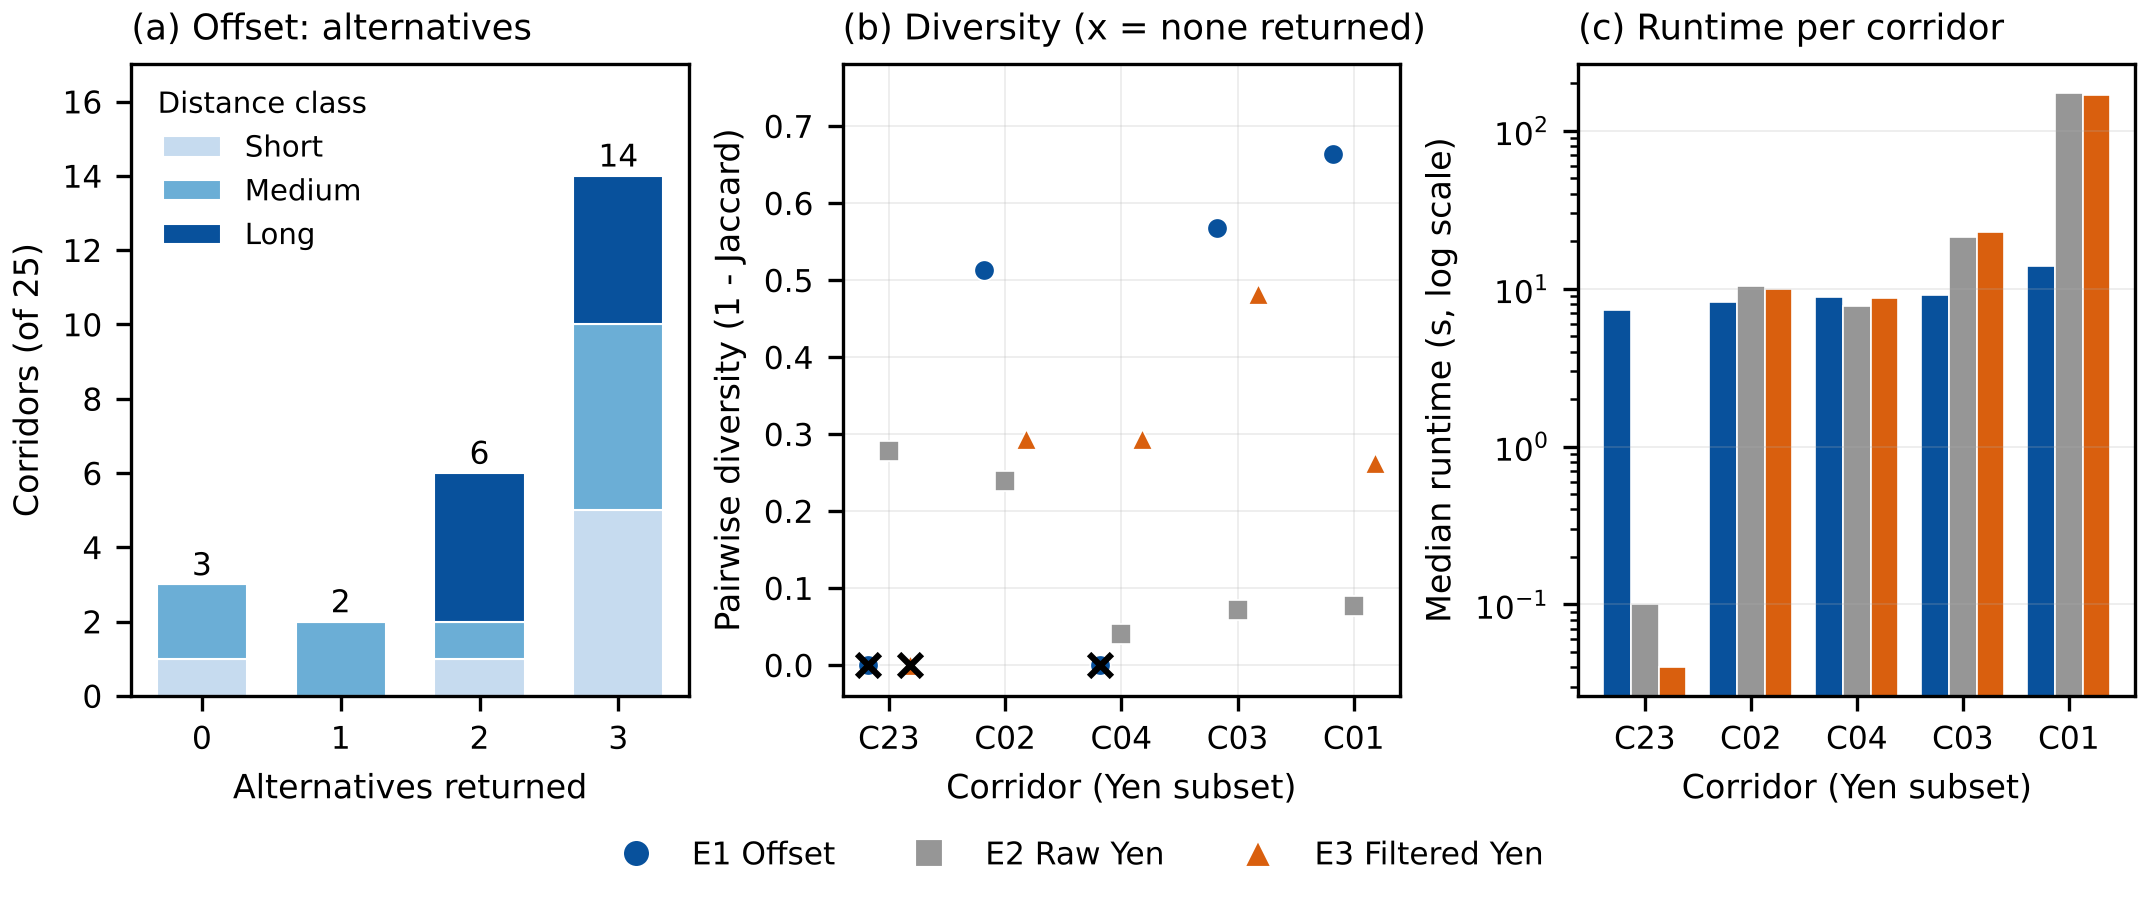
\includegraphics[width=0.94\textwidth]{fig_expE_phase3.png}
\caption{Experiment E evaluation across E1 (Perpendicular Offset, $N=25$), E2 (Raw Yen, $N=5$), and E3 (Filtered Yen, $N=5$). E1 spans all 25 corridors; E2 and E3 evaluate the five-corridor subset. Execution times for E2 and E3 are dominated by OD\_01 (173.6~s and 169.6~s, respectively) and are descriptive.}
\label{fig:expE}
\end{figure*}

\begin{table}[t]
\caption{Experiment E1: Offset Method across 25 Corridors (Measured)}
\label{tab:expE_offset}
\centering
\footnotesize
\setlength{\tabcolsep}{2pt}
\renewcommand{\arraystretch}{1.05}
\begin{tabular}{@{}lrrrrr@{}}
\hline
\textbf{Class} & \textbf{$n$} & \textbf{Any alt.} & \textbf{K=3} & \textbf{Mean alts.} & \textbf{Div.} \\
\hline
Short           & 7  & 6 (85.7\%) & 5 & 2.43 & 0.622 \\
Medium          & 10 & 8 (80.0\%) & 5 & 1.90 & 0.530 \\
Long            & 8  & 8 (100\%)  & 4 & 2.50 & 0.545 \\
\hline
\textbf{All}   & \textbf{25} & \textbf{22 (88.0\%)} & \textbf{14 (56.0\%)} & \textbf{2.24} & \textbf{0.561} \\
\hline
\end{tabular}
\vspace{1.5pt}
\begin{minipage}{\columnwidth}
\scriptsize
\textit{Notes:} Div.: mean pairwise diversity $\mathcal{D}$ (Eq.~\ref{eq:diversity}) on successful corridors ($\ge 1$ alternative); zero-padded mean across all 25 corridors is 0.4932. Runtime: median 9.09~s, mean 10.52~s, range 7.36--22.54~s. Mean detour 1.046; mean overlap 0.496 (56 alternatives). Three corridors (OD\_04, OD\_15, OD\_23) returned zero alternatives.
\end{minipage}
\end{table}

As detailed in Table~\ref{tab:expE_offset} and Fig.~\ref{fig:expE}, the offset method successfully identified valid alternatives on 22 of 25 corridors (88.0\%), reaching the $K=3$ cap on 14 corridors.
All 56 surviving paths satisfied production bounds ($\varepsilon \le 1.1939$, $\gamma \le 0.6911$), achieving an average diversity of 0.5605 on successful corridors (0.4932 zero-padded).
On the three failing corridors (OD\_04, OD\_15, OD\_23), lateral displacement exceeded the 1.20 detour threshold due to severe network bottlenecks.
Median execution time was 9.09~s (range 7.36--22.54~s).

The five-corridor benchmark ($n=5$, descriptive) highlights a coverage-versus-diversity trade-off.
Filtered Yen (E3) achieved broader corridor coverage (mean 2.4 vs.\ 1.2 routes; $K=3$ reached on 4 vs.\ 1 corridor) by exploring the global shortest-path tree, pruning 323 candidates via overlap filtering.
Conversely, on matched corridors where both methods succeeded ($n=3$), the offset method produced substantially higher topological diversity (mean 0.58 vs.\ 0.35) and lower overlap (0.44 vs.\ 0.53).
Raw Yen (E2) produced near-duplicate routes (overlap 0.93, diversity 0.13).
Mean execution times (E1: 9.5~s; E2: 42.6~s; E3: 41.5~s) were heavily skewed by OD\_01; Yen ran faster on two corridors, so no general speed-up is asserted.

\subsection{Pilot External Comparison}

\begin{figure*}[t]
\centering
\begin{minipage}[t]{0.32\textwidth}
  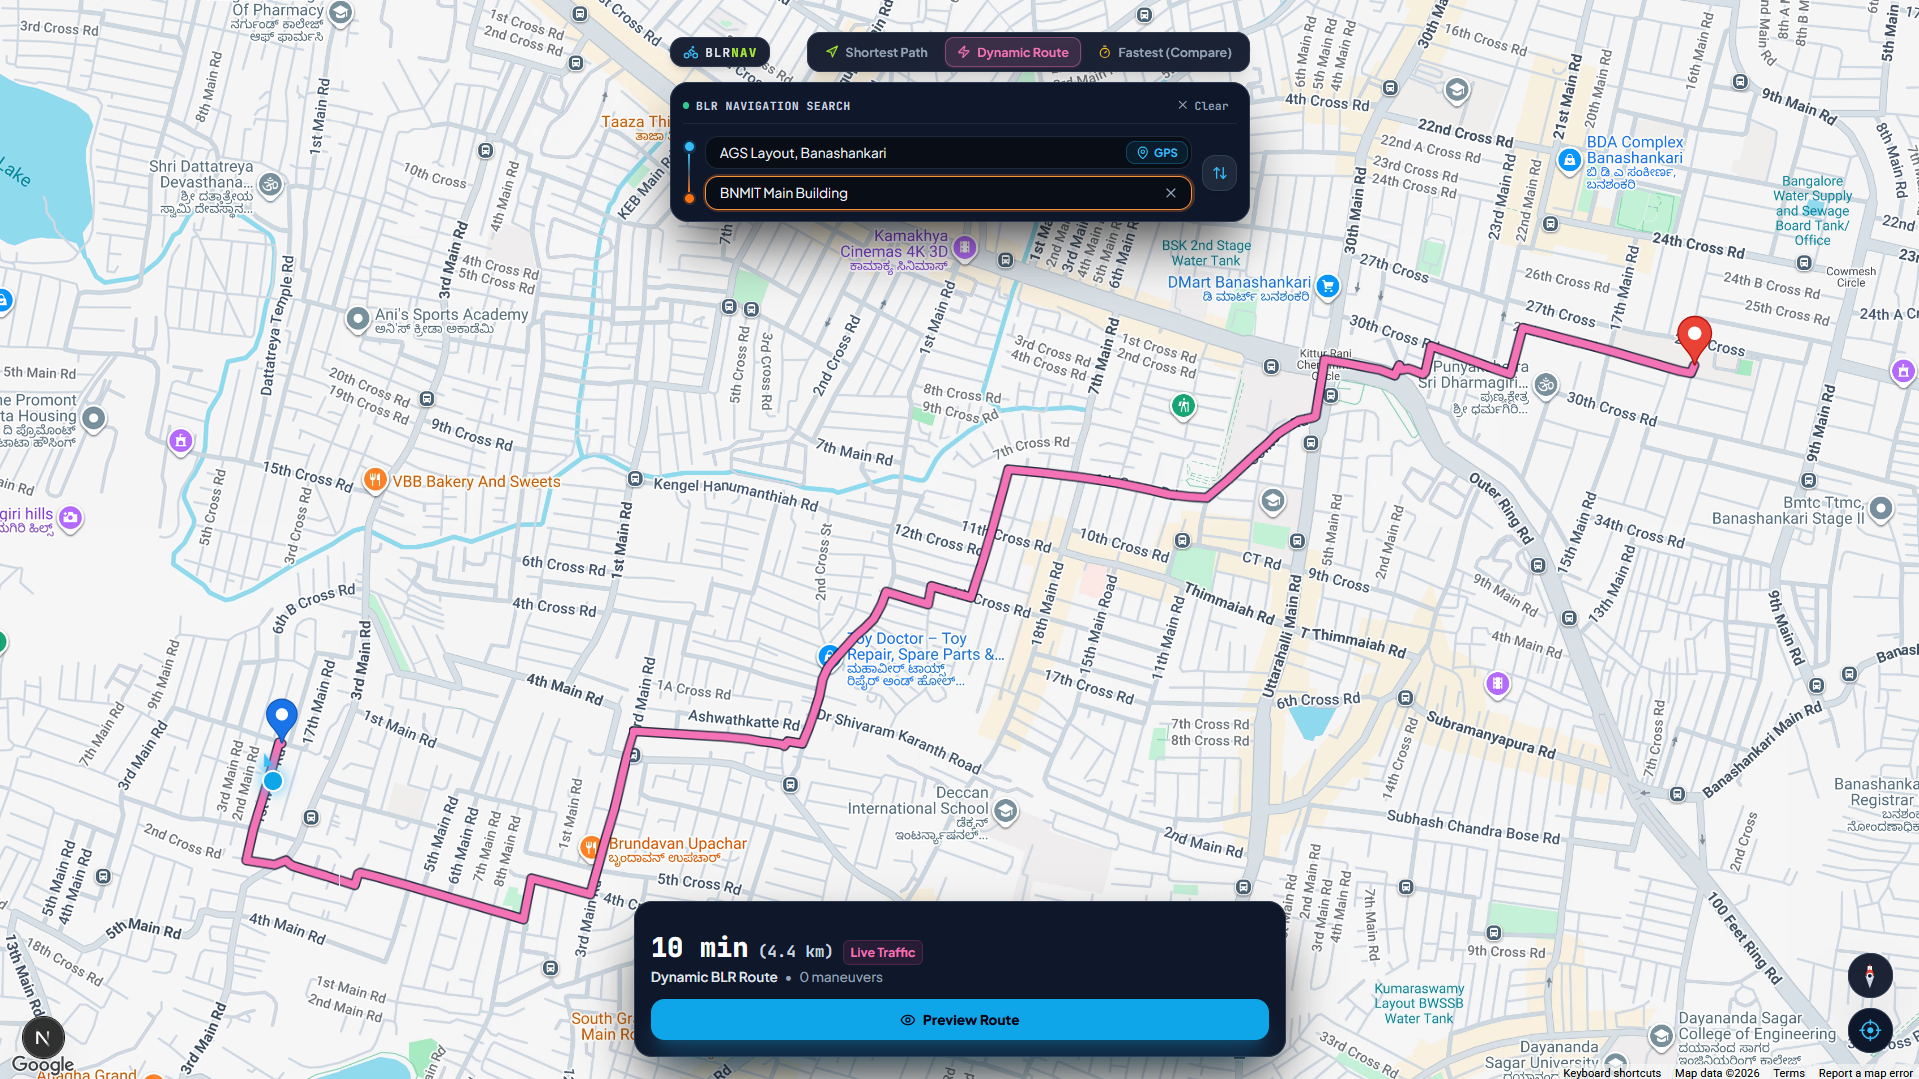
\includegraphics[width=\linewidth]{pair_b_project.png}
  \centerline{\footnotesize (a) Routing framework (Dynamic mode)}
\end{minipage}\hfill
\begin{minipage}[t]{0.32\textwidth}
  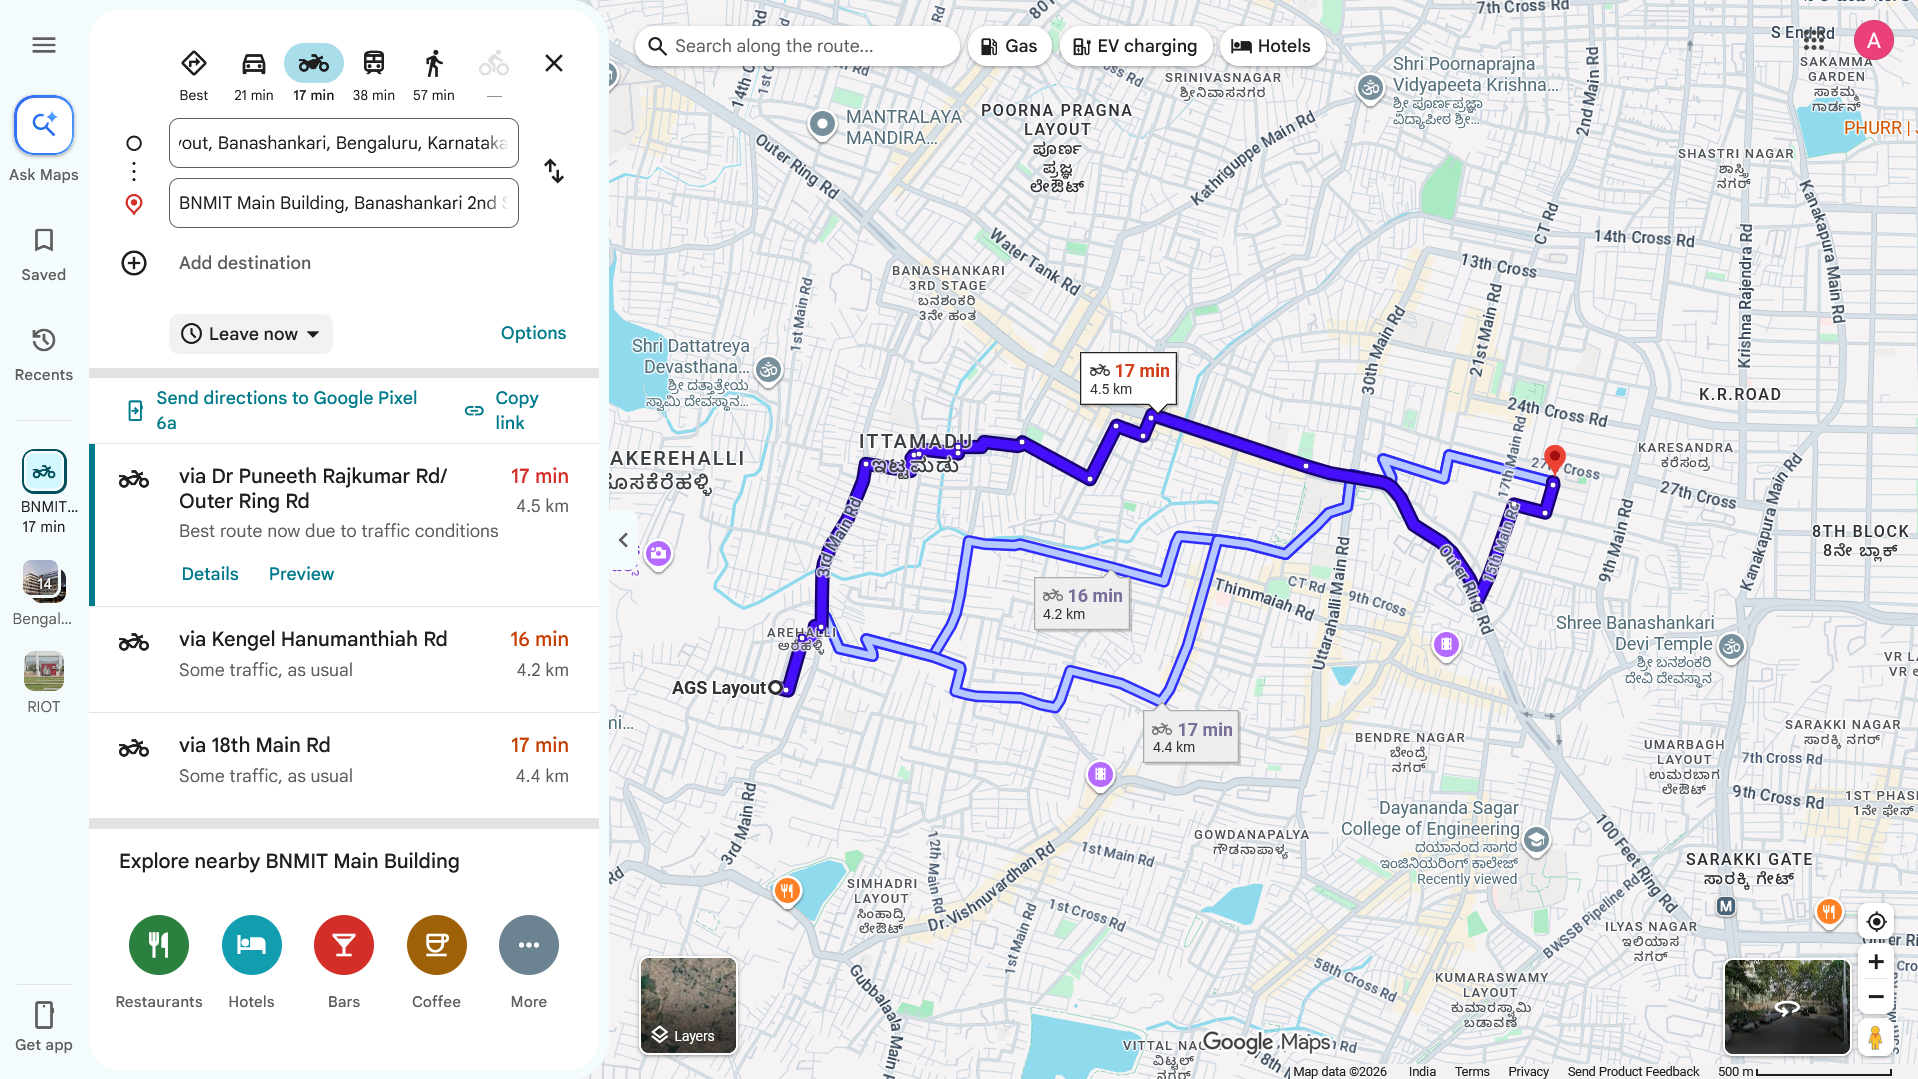
\includegraphics[width=\linewidth]{pair_b_gmaps.png}
  \centerline{\footnotesize (b) Google Maps (motorcycle tab)}
\end{minipage}\hfill
\begin{minipage}[t]{0.32\textwidth}
  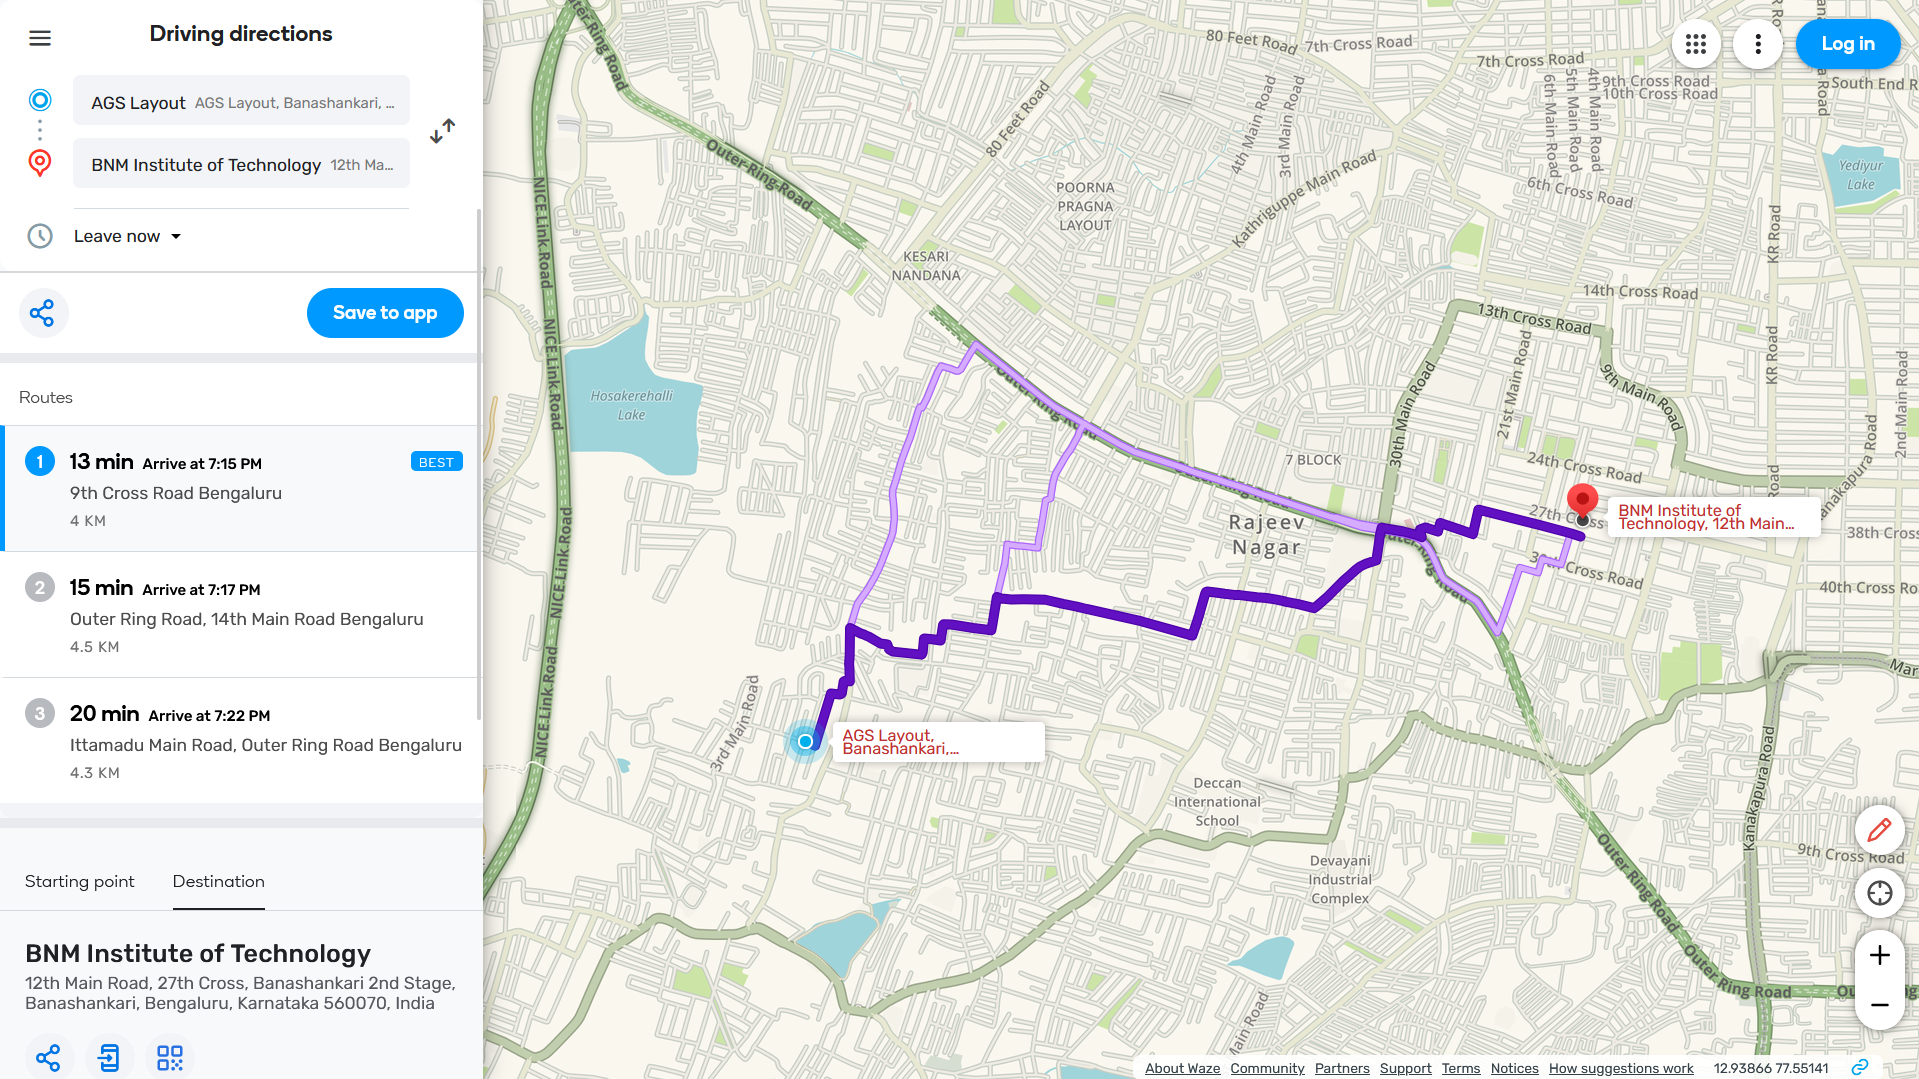
\includegraphics[width=\linewidth]{pair_b_waze.png}
  \centerline{\footnotesize (c) Waze (motorcycle vehicle type)}
\end{minipage}
\caption{Pilot Pair~B visual interface captures: routing framework (Dynamic mode), Google Maps (motorcycle tab), and Waze (motorcycle type). Images display third-party map tiles and place names; precise coordinates remain confidential. The routing framework outputs a single route by design, whereas Google Maps and Waze present three alternatives.}
\label{fig:pilot_case}
\end{figure*}

\begin{table}[t]
\caption{Pilot Comparison: Pairs A to D (Measured from Screenshots)}
\label{tab:pilot}
\centering
\footnotesize
\setlength{\tabcolsep}{2pt}
\renewcommand{\arraystretch}{1.05}
\begin{tabular}{@{}lcrrrrrr@{}}
\hline
\textbf{Pair} & \textbf{Class} & \multicolumn{2}{c}{\textbf{Framework}} & \multicolumn{2}{c}{\textbf{Google Maps}} & \multicolumn{2}{c}{\textbf{Waze}} \\
 & & km & min & km & min & km & min \\
\hline
A & Long   & 24.2 & 53 & 33.7 & 65 & 21.7 & 62 \\
B & Short  &  4.4 & 10 &  4.5 & 17 &  4.0 & 13 \\
C & Long   & 17.4 & 59 & 15.6 & 65 & 14.6 & 75 \\
D & Medium & 13.2 & 41 & 16.8 & 52 & 17.4 & 55 \\
\hline
\end{tabular}
\vspace{1.5pt}
\begin{minipage}{\columnwidth}
\scriptsize
\textit{Notes:} Four pairs captured in one evening window. Waze motorcycle mode is user-confirmed. Framework ETAs are derived via Google Routes API via-waypoints (non-independent). Pair~A Waze route flagged toll usage. No physical travel was conducted; metrics are model predictions only.
\end{minipage}
\end{table}

Table~\ref{tab:pilot} and Fig.~\ref{fig:pilot_case} report visual interface comparisons across Pairs A--D.
The framework returns one route per request by design; commercial platforms display multiple alternatives.
Values reflect divergent geocoding, base networks, and traffic feeds; they cannot be treated as equivalent measurements.
Because framework ETAs rely on Google Routes API queries, they share provenance with Google estimates.
No platform ranking or performance superiority is asserted.

\subsection{Strava Journey Analysis}

\begin{figure*}[t]
\centering
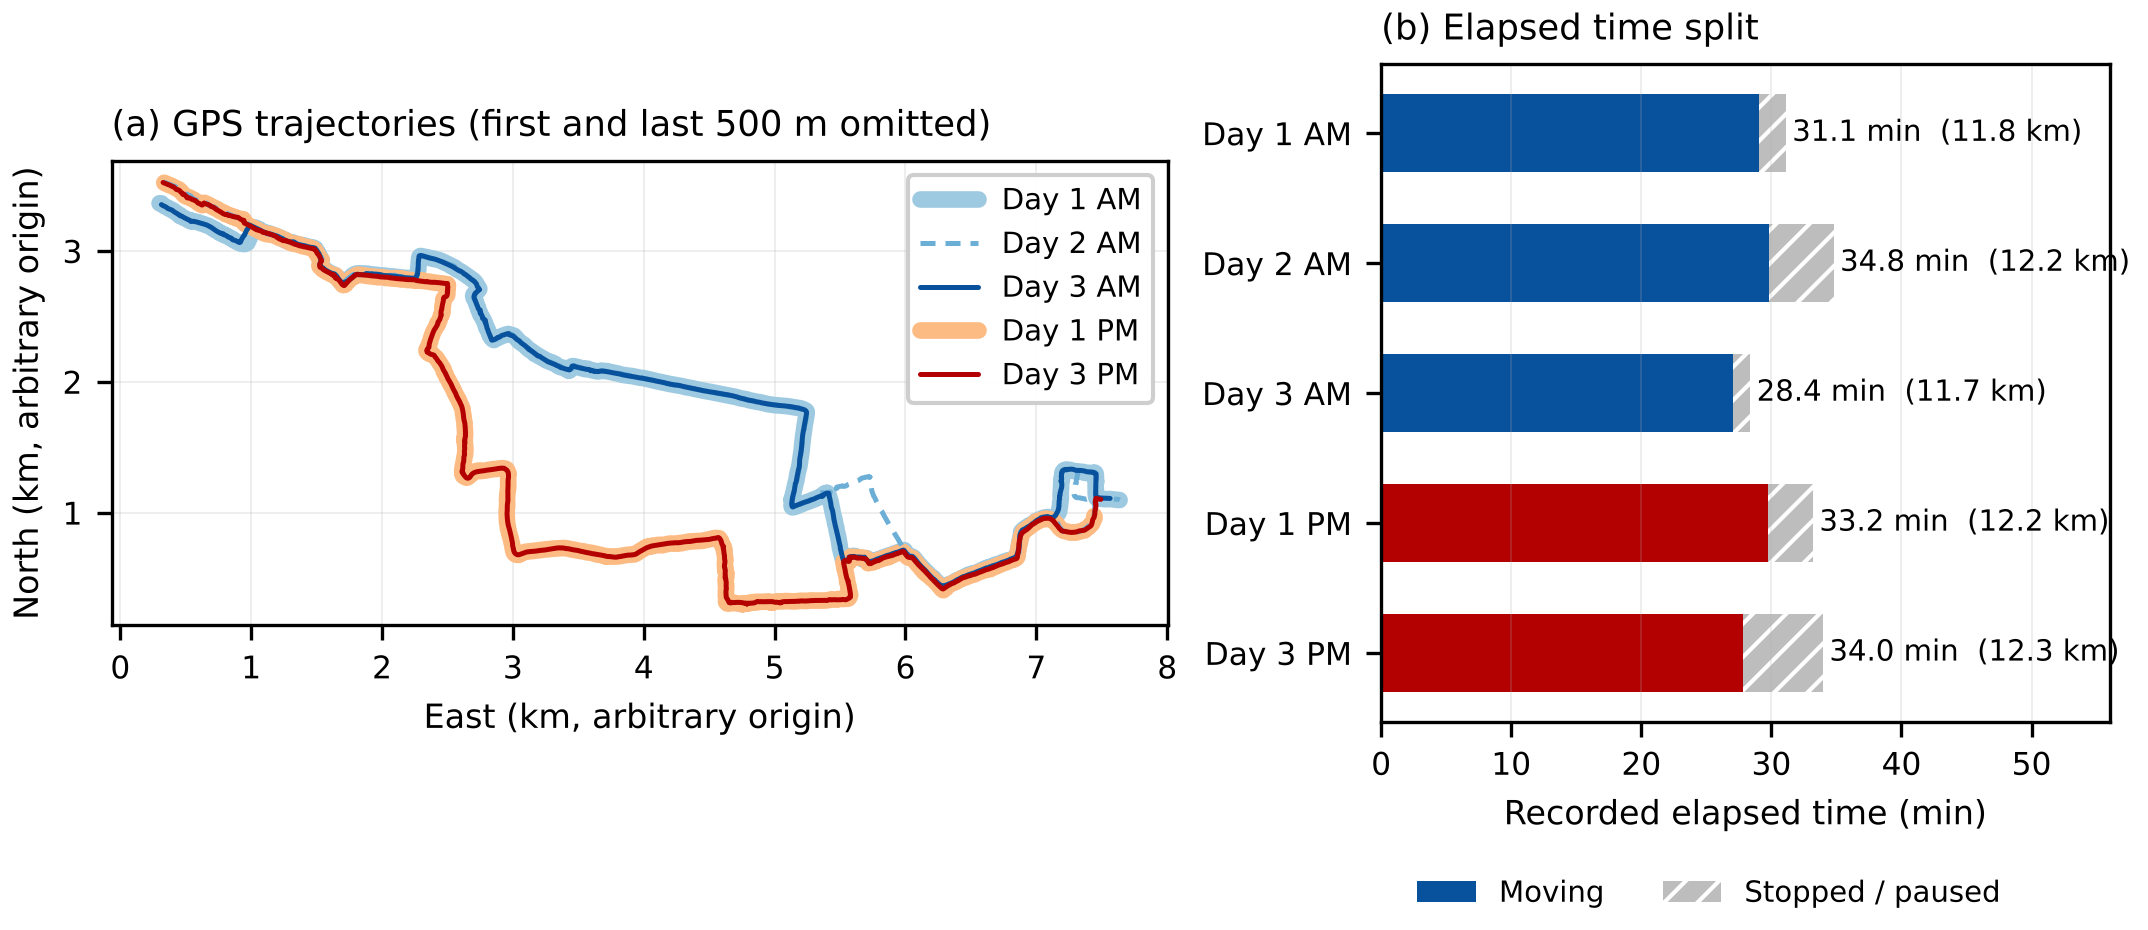
\includegraphics[width=0.94\textwidth]{fig_strava_phase2.png}
\caption{GPS trajectory analysis across five rides on three days. Top: anonymised trajectories in arbitrary-origin meters with the first and last 500~m excluded; morning (AM) and afternoon (PM) rides displayed separately. Bottom: stacked time breakdown (moving vs.\ stopped, threshold 0.50~m/s) per ride. Coordinates and timestamps are removed; raw GPX files remain in the author's private archive.}
\label{fig:strava}
\end{figure*}

\begin{table}[t]
\caption{Strava Ride Summary: Five Rides Across Three Days (Measured from GPX)}
\label{tab:strava}
\centering
\footnotesize
\setlength{\tabcolsep}{2pt}
\renewcommand{\arraystretch}{1.05}
\begin{tabular}{@{}lrrrrr@{}}
\hline
\textbf{Ride} & \textbf{Dist.\ (km)} & \textbf{Elapsed (min)} & \textbf{Moving (min)} & \textbf{Stopped (min)} & \textbf{Stops} \\
\hline
Day 1 AM & 11.84 & 31.1 & 29.1 & 2.1 & 23 \\
Day 2 AM & 12.19 & 34.8 & 29.9 & 4.9 & 26 \\
Day 3 AM & 11.69 & 28.4 & 27.0 & 1.4 & 13 \\
Day 1 PM & 12.20 & 33.2 & 29.7 & 3.5 & 23 \\
Day 3 PM & 12.29 & 34.0 & 27.8 & 6.1 & 21 \\
\hline
\end{tabular}
\vspace{1.5pt}
\begin{minipage}{\columnwidth}
\scriptsize
\textit{Notes:} Stopped threshold: 0.50~m/s. Recording start and end locations varied slightly across rides; raw lengths are not directly comparable. Vehicle: two-wheeler. Elapsed times reflect traffic and cannot be compared against model ETAs. Stopped durations vary by 0.5--2.3~min across threshold sensitivity range (0.30--1.00~m/s).
\end{minipage}
\end{table}

Table~\ref{tab:strava} and Fig.~\ref{fig:strava} report trajectory consistency across five GPS rides on three days.
Morning journeys on Day~1 and Day~3 followed near-identical routes: mean deviation was 3.4~m (P90 6.2~m, max 50.9~m; 98.1\% within 15~m; \textbf{Measured}).
Afternoon journeys on Day~1 and Day~3 exhibited comparable repeatability: mean deviation was 2.9~m (P90 6.2~m, max 18.6~m; 99.8\% within 15~m; \textbf{Measured}).
The Day~2 morning trip diverged from the baseline path (mean $\approx 59$~m, P90 215~m, max 443~m; cause unverified).
A control comparison between Day~1 morning and afternoon paths yielded 377~m mean divergence, confirming that the metric reliably separates distinct paths.
The afternoon trajectory was recommended by the framework during a rerouting event and executed on Day~1 and Day~3 (\textbf{User-confirmed}).
The morning baseline route represents a \textbf{Recovered historical snapshot}; contemporaneous display was not independently validated.

% ============================================================
% VI. DISCUSSION AND LIMITATIONS
% ============================================================

\section{Discussion and Limitations}

\noindent\textbf{Coverage and Topological Trade-offs:}
The offset method achieves an 88.0\% corridor success rate, demonstrating that lateral waypoint displacement effectively identifies viable alternatives across typical urban layouts.
On corridors with severe topological barriers (such as OD\_04, OD\_15, and OD\_23), lateral excursions consistently exceed the 1.20 detour limit, returning no valid alternative.
Filtered Yen circumvents this geometric constraint by traversing the global shortest-path tree, albeit at the cost of higher edge overlap and lower spatial separation.
The five-corridor subset ($n=5$) illustrates this trade-off but remains purely descriptive.

\noindent\textbf{Platform Evaluation and Independence:}
The pilot study is restricted to four corridor pairs evaluated within a single evening window.
Commercial platforms rely on distinct road networks, proprietary geocoding, and independent traffic inputs.
Because framework ETAs are generated by querying the Google Routes API with framework path waypoints, the two services are not independent estimators.
Waze motorcycle settings are user-confirmed and not visible in archived screenshots.
These pilot observations document operational feasibility but do not establish platform rankings or travel-time superiority.

\noindent\textbf{Empirical Trajectory Constraints:}
The empirical GPS corpus represents a single rider across three days on one origin-destination pair.
Variations in trip start and end locations preclude raw distance comparisons.
Total elapsed times (28.4--34.8~min) reflect traffic delays, signal stops, and rider behavior; they cannot validate algorithmic ETAs.
Stopped-time classifications are sensitive to velocity thresholds, shifting by 0.5--2.3~min across the 0.30--1.00~m/s range.
No definitive cause for the Day~2 morning detour can be confirmed.

\noindent\textbf{Network Assumptions and Future Directions:}
Network analysis is restricted to a static OpenStreetMap snapshot of Bengaluru; unmapped infrastructure or subsequent modifications are omitted.
Turn deflection angles are derived from street centerline vectors and do not capture dynamic police diversions or temporary blockages.
Graph traversal impedance serves as a search cost rather than a calibrated measure of physical duration or energy consumption.
The signal-delay discount formulation present in experimental stubs was uninvoked in production runs and is excluded from all reported results \cite{promraksa2022lane,abbas2019internet}.
Future research will investigate multi-city generalisation, real-time dynamic graph updates, rider preference calibration, and IoT traffic sensing integration \cite{abbas2019internet}.

% ============================================================
% VII. CONCLUSION
% ============================================================

\section{Conclusion}

This paper presented and evaluated an independent two-wheeler routing framework combining turn-aware state-expanded $A^*$ search with Shortest and Dynamic operational modes and a perpendicular-offset alternative-route generator.
Across 25 Bengaluru corridors, the offset generator produced valid alternatives ($\varepsilon \le 1.20$, $\gamma \le 0.70$) on 22 corridors (88.0\%), achieving an average pairwise diversity of 0.5605 on successful corridors.
A descriptive five-corridor benchmark against filtered Yen revealed a fundamental coverage-versus-diversity trade-off.
Manual pilot observations documented comparative platform metrics without asserting rankings, and repeat GPS journeys demonstrated spatial path consistency across multiple days.
No travel-time savings, safety improvements, or platform superiority are claimed; all findings constitute descriptive empirical measurements on an urban road network.

\balance
\bibliographystyle{IEEEtran}
\bibliography{paper2_verified_references}

\end{document}
